\documentclass[compress]{beamer}

\mode<presentation>
\usetheme{Madrid}
\definecolor{Columbia}{RGB}{185,217,235}
\definecolor{Columbia2}{RGB}{0,51,160}
\definecolor{Columbia3}{RGB}{0,114,206}
\setbeamercolor{title}{fg=Columbia2}
\setbeamercolor{frametitle}{fg=Columbia2}
\setbeamercolor{block title}{bg=Columbia, fg=Columbia2}
%\setbeamercolor{block body}{fg=Columbia2}
\setbeamercolor{structure}{fg=Columbia}
\setbeamercolor{item projected}{fg=white}
\setbeamercolor{item}{fg=Columbia2}
\setbeamercolor{subitem}{fg=Columbia2}
\setbeamercolor{section in toc}{fg=Columbia2}
\setbeamercolor{description item}{fg=Columbia}
\setbeamercolor{caption name}{fg=Columbia2}
\setbeamercolor{button}{fg=Columbia2}
\usepackage{graphics}
\usepackage{geometry}
\usepackage{booktabs}
\usepackage{tikz}
\usepackage{amsmath}
\usepackage{bbm}
\usetikzlibrary{decorations.pathreplacing}
\usepackage{multirow, makecell}
\usepackage{float}
\usepackage{fancyvrb}
\usepackage{caption}
\usepackage{subcaption}
\usepackage{adjustbox}
\usepackage{threeparttable}
\usepackage{hyperref}
\usepackage[scaled=0.92]{helvet}
\newenvironment{wideitemize}{\itemize\addtolength{\itemsep}{10pt}}{\enditemize}
\newenvironment{wideenumerate}{\enumerate\addtolength{\itemsep}{10pt}}{\endenumerate}
%\hypersetup{
%colorlinks=true,
%linkcolor=black,
%filecolor=green, 
%urlcolor=blue,
%}
\beamertemplatenavigationsymbolsempty
\setbeamercolor{author in head/foot}{bg=Columbia2, fg=white}
\setbeamercolor{title in head/foot}{bg=Columbia3, fg=white}
\setbeamercolor{date in head/foot}{bg=Columbia, fg=Columbia2}
\setbeamercolor{section in head/foot}{bg=Columbia, fg=Columbia2}
\setbeamercolor{headline}{bg=Columbia}
\setbeamertemplate{footline}{
    \leavevmode%
    \hbox{%
        \begin{beamercolorbox}[wd=.333333\paperwidth,ht=2.25ex,dp=1ex,center]{author in head/foot}%
            \usebeamerfont{author in head/foot}\insertshortauthor
        \end{beamercolorbox}%
        \begin{beamercolorbox}[wd=.333333\paperwidth,ht=2.25ex,dp=1ex,center]{title in head/foot}%
            \usebeamerfont{title in head/foot}\insertshorttitle
        \end{beamercolorbox}%
        \begin{beamercolorbox}[wd=.333333\paperwidth,ht=2.25ex,dp=1ex,right]{date in head/foot}%
            \usebeamerfont{date in head/foot}\insertshortdate{}\hspace*{2em}
            \insertframenumber{} / \inserttotalframenumber\hspace*{2ex} 
        \end{beamercolorbox}}%
        \vskip0pt%
    }
\setbeamercolor{page number in head/foot}{fg=black}
\setbeamertemplate{section in toc}[sections numbered]
\setbeamertemplate{subsection in toc}{\leavevmode\leftskip=3em\rlap{\hskip-1.75em\inserttocsectionnumber.\inserttocsubsectionnumber}\inserttocsubsection\par}
\setbeamerfont{subsection in toc}{size=\footnotesize}
%\setbeamertemplate{headline}{%
  %\begin{beamercolorbox}[ht=5.5ex]{section in head/foot}
    %\vskip2pt\insertnavigation{0.33\paperwidth}\vskip2pt
  %\end{beamercolorbox}%
%}


\makeatletter
\let\@@magyar@captionfix\relax
\makeatother


\title[Recitation 5]{Recitation 5} % Change this regularly
\author[Seung-hun Lee]{Seung-hun Lee}
\institute[Columbia University]{Columbia University}

\date[]{}

\begin{document}
\begin{frame}
\titlepage
\end{frame}

%%%%%%%%%%%%% Section 1. 


% Capture in one slide
% Separate slide for questions
\begin{frame}
\frametitle{Multivariate Regression Models}
Sampling distribution 
\begin{itemize}
\item The estimates for the $\hat{\beta}_j$, can be obtained in a similar way in which we have obtained the OLS estimates for the single variable version.
\[
\min_{\{\beta_0,\beta_1,\beta_2\}} \sum_{i=1}^n[Y_i-\beta_0 - \beta_1X_{1i}-\beta_2X_{2i}]^2
\]
\item After some more amount of algebra (than the single variable case), the result we get is the following
\begin{itemize}
\item[$\hat{\beta}_0=$] $\bar{Y}-\hat{\beta}_1\bar{X}_1-\hat{\beta}_2\bar{X}_2$
\item[$\hat{\beta}_1=$] $\frac{\sum_{i=1}^n (X_{1i}-\bar{X}_1)(Y_{i}-\bar{Y})\sum_{i=1}^n(X_{2i}-\bar{X}_2)^2-\sum_{i=1}^n (X_{2i}-\bar{X}_2)(Y_{i}-\bar{Y})\sum_{i=1}^n(X_{1i}-\bar{X}_1)(X_{2i}-\bar{X}_2)}{\sum_{i=1}^n (X_{1i}-\bar{X}_1)^2\sum_{i=1}^n (X_{2i}-\bar{X}_2)^2-[\sum_{i=1}^n (X_{1i}-\bar{X}_1)(X_{2i}-\bar{X}_2)]^2}$
\item[$\hat{\beta}_2=$] $\frac{\sum_{i=1}^n (X_{2i}-\bar{X}_2)(Y_{i}-\bar{Y})\sum_{i=1}^n(X_{1i}-\bar{X}_1)^2-\sum_{i=1}^n (X_{1i}-\bar{X}_1)(Y_{i}-\bar{Y})\sum_{i=1}^n(X_{1i}-\bar{X}_1)(X_{2i}-\bar{X}_2)}{\sum_{i=1}^n (X_{1i}-\bar{X}_1)^2\sum_{i=1}^n (X_{2i}-\bar{X}_2)^2-[\sum_{i=1}^n (X_{1i}-\bar{X}_1)(X_{2i}-\bar{X}_2)]^2}$
\end{itemize} \par\medskip
\item What matters at this point is how we should \textbf{interpret} these coefficients. 
\end{itemize}
\end{frame}

\begin{frame}
\frametitle{Multivariate Regression Models}
Multicollinearity
\begin{itemize}
\item We are quite likely to end up including independent variables that are highly correlated with each other. There are two \item We say two variables $X_1$ and $X_2$ are \textbf{perfectly multicollinear} if $X_1$ is in an exact linear relationship of some sort with $X_2$.
\item Any multicollinearities that are not in exact linear relationship is referred to as \textbf{imperfect multicollinearity}. 
\end{itemize}
\end{frame}

\begin{frame}
\frametitle{Multivariate Regression Models}
Multicollinearity
\begin{itemize}
\item \textbf{Assume that $X_2 = cX_1$ for some constant $c$}: Then we have $(X_{2i}-\bar{X}_2)=c(X_{1i}-\bar{X}_1)$. Then $\hat{\beta}_1$ changes to $\frac{0}{0} $ 
\item \textbf{Dummy variable trap}: Say that you have the dummy variable for females and males. Let each of them be $X_{1i}$ and $X_{2i}$ with $X_{2i}=1-X_{1i}$. Then the regression can be written as
\begin{gather*}
Y_i = \beta_0 + \beta_1X_{1i} + \beta_2X_{2i} + u_i \iff Y_i = \beta_0 + \beta_1X_{1i} + \beta_2(1-X_{1i}) + u_i \\
\iff Y_i = \beta_0 + \beta_2 +(\beta_1-\beta_2)X_{1i}+u_i
\end{gather*}
Therefore, by including both $X_{1i}$ and $X_{2i}$ in the same regression, the $X_{2i}$ vanishes from the equation. This is why when you have dummy variables for all categories in the observation, \textbf{one of them must be left out.}
\end{itemize}
\end{frame}


\begin{frame}
\frametitle{Multivariate Regression Models}
Joint hypothesis tests (Why it is not straightforward)
\begin{itemize}
\item Suppose that you are running a two-sided test with 5 independent variables and significance level $\alpha = 5\%$ under the null hypothesis
\[
H_0: \beta_1=...\beta_5=0
\]
\item You reject the null hypothesis when $|t_i|\geq 1.96 $ with probability 0.05. 
\item Now assume that each test statics are independent. Then the probability of incorrectly rejecting the null hypothesis using this approach is
\footnotesize{\[
\begin{aligned}
\Pr(|t_1|>1.96 \cup...\cup |t_5|>1.96) & =1-\Pr(|t_1|\leq1.96\cap .. \cap|t_1|\leq1.96)\\
(\because\text{Independence of $t_i$'s}) \ \ &=1-\Pr(|t_1|\leq1.96)\times ..\times\Pr(|t_5|\leq1.96) \\
 & = 1-(0.95)^5 \\
 &= 0.2262
\end{aligned}
\]}\normalsize
\item This means that the rejection rate under the null is not 5\% but 22\% percent - we end up rejecting the null hypothesis more than we have to.
\end{itemize}
\end{frame}


\begin{frame}
\frametitle{Multivariate Regression Models}
F-test
\begin{itemize}
\item This is a test where all parts of the joint hypothesis can be tested at once. It also has mechanism for correcting the correlation between the $t$-test statistics.
\item It ultimately allows us to correctly set the significance level even for the multiple testing case.
\item The usual joint hypothesis test for the regression with $k$ variables (not including the constant term) is
\[
H_0: \beta_1 = ... =\beta_k=0, \ H_1:\lnot H_0
\]
where $H_1$ refers to the case where there is a nonzero element in any one of $\beta_1$ to $\beta_k$.
\item Note that the default F-test null hypothesis for STATA is as above
\end{itemize}
\end{frame}


\begin{frame}
\frametitle{Multivariate Regression Models}
Other tests
\begin{itemize}
\item Suppose that instead of $\beta_1$ and $\beta_2$ being zero, we are just interested in whether they are equal.
\item The $F$-test can also be used for testing this hypothesis. The setup of the hypothesis would be
\[
H_0: \beta_1 = \beta_2 \ H_1: \beta_1 \neq \beta_2
\]
\item With this, you can answer various types of tests (e.g. is $\beta_1+\beta_2=100$?)
\end{itemize}
\end{frame}

\begin{frame}
\frametitle{Multivariate Regression Models}
Interpreting the results
\begin{itemize}
\item Below are the results of a sample regression on multiple variables. I regress \textit{birthweight} on \textit{smoker, alcohol, Nprevist} (number of prenatal visits to doctor).
\begin{figure}[H]
\begin{center}
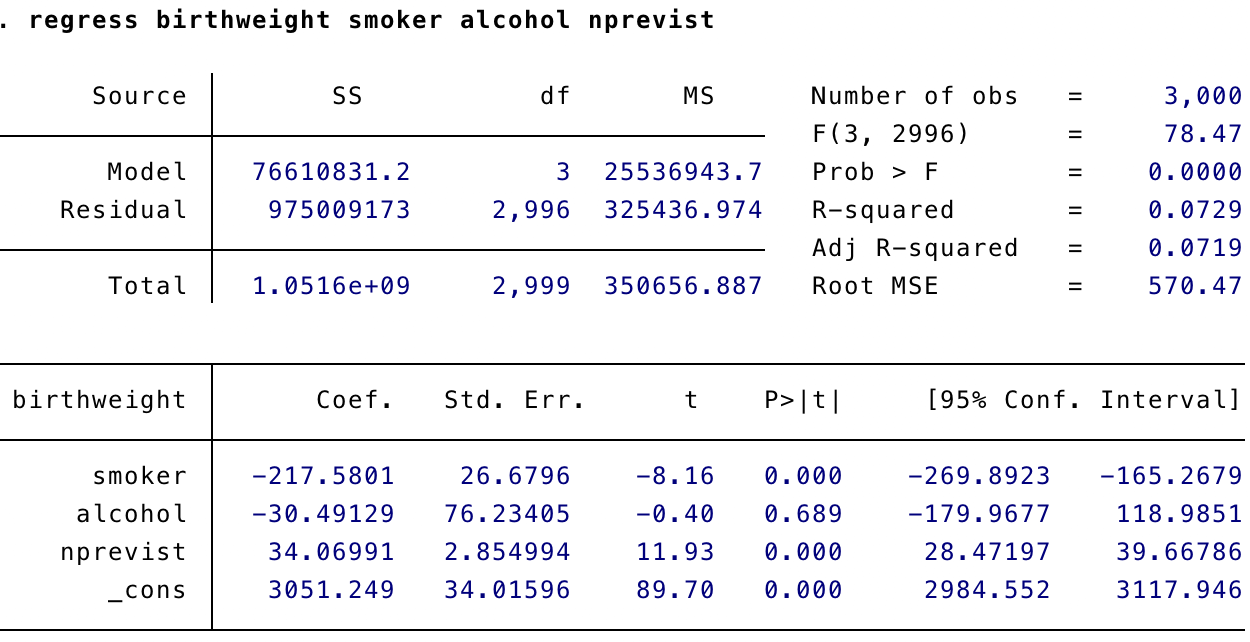
\includegraphics[width=0.7\textwidth]{regoutput.png}
\end{center}
\end{figure}\par\medskip
\item You can see that running multivariate regression is similar in terms of the techniques involved.
\end{itemize}
\end{frame}

\begin{frame}
\frametitle{Multivariate Regression Models}
Interpreting the results
\begin{itemize}
 \item Additional complication rises from interpreting the goodness of fit. In addition to $R^2$, we now get the \textbf{adjusted $R^2$}, which is defined as
\[
\bar{R}^2 = 1-\frac{n-1}{n-k-1}\frac{\text{RSS}}{\text{TSS}}
\]
\item Since we are assuming that $k\geq 1$, adjusted $R^2$ is smaller than the $R^2$. 
\item As we include more variables, the $\frac{n-1}{n-k-1}$ increases, leading to further decrease in adjusted $R^2$. \item However, if the new variables are very relevent, $\frac{\text{RSS}}{\text{TSS}}$ decreases. 
\item This reduces the gap between $R^2$ and the adjusted $R^2$. If the adjusted $R^2$ do not decrease drastically, it is a sign that we are adding a relevant variable. \par\medskip
\end{itemize}
\end{frame}


\begin{frame}
\frametitle{Multivariate Regression Models}
Deriving The $F$-statistic
\begin{itemize}
 \item One uses $t$-statistics from individual hypotheses. This is calculated as
\[
\frac{1}{2}\left(\frac{t_1^2+t_2^2-2\hat{\rho}_{t_1,t_2}t_1t_2}{1-\hat{\rho}^2_{t_1,t_2}}\right)
\]\
\item Another, which is useful for calculating $H_0: \beta_1 = ... =\beta_q=0$ hypothesis, uses $R^2$ from the 'unrestricted' and 'restricted' regressions.
\begin{itemize}
\item Assume the following setup
\footnotesize{\[\begin{aligned}
\text{Restricted: } & Y_i =\beta_0+ 0X_{1,i} + ...+ 0X_{q,i}+ \beta_{q+1}X_{q+1,i}+...+\beta_kX_{k,i} + u_i\\
\text{Unrestricted: } & Y_i = \beta_0+\beta_1X_{1,i} + ... +\beta_qX_{q,i}+ \beta_{q+1}X_{q+1,i}+...+\beta_kX_{k,i} + u_i\\
\end{aligned}\]}\normalsize
\item Restricted regression assumes that $H_0$ is true and then only optimizes with respect to $\beta_{q+1},...,\beta_{k}$.
\item Unrestricted regression does not assume that $H_0$ is true and optimizes with respect to all slope coefficients.
\end{itemize}
\end{itemize}
\end{frame}


\begin{frame}
\frametitle{Multivariate Regression Models}
Deriving The $F$-statistic
\begin{itemize}
 \item We use $R^2$ from these two regressions. 
\[
\frac{(R^2_{\text{Unrestricted}}-R^2_{\text{Restricted}})/q}{(1-R^2_{\text{Unrestricted}})/(n-k-1)}
\]
\begin{itemize}
\item $k$: number of independent variables (not counting intercept)
\item $q$ is the number of restrictions. 
\item Since unrestricted models allows roles for $X_1,...,X_q$ variables, they have higher $R^2$ (Restricted: They should have no role)
\end{itemize}
\item Another: Using $R^2_{\text{Restricted}} = 1-\frac{RSS_{\text{Restricted}}}{TSS}$, we can write
\[
\frac{(RSS_{\text{Restricted}}-RSS_{\text{Unrestricted}})/q}{(RSS_{\text{Unrestricted}})/(n-k-1)}
\] 
\end{itemize}
\end{frame}

\begin{frame}
\frametitle{Multivariate Regression Models}
Control variables and conditional mean independence
\begin{itemize}
 \item Assume that 
 \[
\begin{aligned}
\text{True: }& Y_i = \beta_0 + \beta_1 X_i + \beta_2 Z_i+u_i\\
\text{Mistake: }& Y_i = \beta_0 + \beta_1 X_i + u_i^*\\
\text{Sample: }& Y_i = \hat{\beta}_0 + \hat{\beta}_1 X_i+ \hat{u}_i\\
\end{aligned}
\]
\item If we end up with an omitted variable bias by not including $Z_i$, Then, we have a problem. 
\[
\begin{aligned}
E[u_i^*|X_i]&=E[\beta_2Z_i+u_i|X_i]\\
&=\beta_2Z_i+E[u_i|X_i] \neq 0
\end{aligned}
\]
\item Assumption 2 from the classical linear regression model (refer to Recitation 3), fails and $\hat{\beta}_1$ without inclusion of $Z_i$ is biased
\end{itemize}
\end{frame}

\begin{frame}
\frametitle{Multivariate Regression Models}
Control variables and conditional mean independence
\begin{itemize}
 \item We can find $W_i$ variable correlated with $Z_i$ and put it in the regression
 \item By doing so, we achieve three things
\begin{itemize}
\item The $u_i$ term is no longer correlated with $X_i$ ($cov(X_i, u_i)=0$)
\item For given value of $W_i$, then the variable of interest $X_i$ is no longer correlated with the omitted determinant of $Y_i$
\item For given $W_i$, $X_i$ acts as if they are randomly assigned
\end{itemize}
\item Variable $W_i$ that achieves this is called an \textbf{effective control variable}. 
\item In this case, we say that the \textbf{conditional mean independence} hold, 
\[
E[u_i|X_i,W_i]= E[u_i|W_i]
\]
\item Note that $W_i$ itself does not need to have causal relationship with $Y_i$

\end{itemize}
\end{frame}

\begin{frame}
\frametitle{Multivariate Regression Models}
Nonlinear regressions
\begin{itemize}
 \item Not everything in world is linearly related
 \item For correlations like this, nonlinear regressors are necessary
 \item When incorporating such regressors, the interpretation of each coefficient becomes trickier.
 \item Quadratic relations: Think about wage and age - wages increase with age, but (usually) at a decreasing pace
 \[
W = \beta_0 + \beta_1 X+ \beta_2 X^2+u
\]
\item The marginal effect of $X$ on $W$ can be written as
\[
\frac{\partial W}{\partial X}=\beta_1+2\beta_2 X
\]
\end{itemize}
\end{frame}

\begin{frame}
\frametitle{Multivariate Regression Models}
Nonlinear regressions
\begin{itemize}
 \item In a linear regressor only format, the marginal effect is
 \[
W = \beta_0 + \beta_1 X+u
\]
\[
\frac{\partial W}{\partial X}=\beta_1
\]
\item The difference is that with quadratic terms, we can express cases where \textit{marginal} changes to $W$ with respect to $X$ is not a constant, but depends on some value of $X$
\begin{itemize}
\item In the above case, if $\beta_2>0$, marginal increase in $W$ increases with $X$ (and vice versa)
\end{itemize}
\end{itemize}
\end{frame}
%%%%%%%%%%%
\end{document}
